\subsection{Class Diagram}

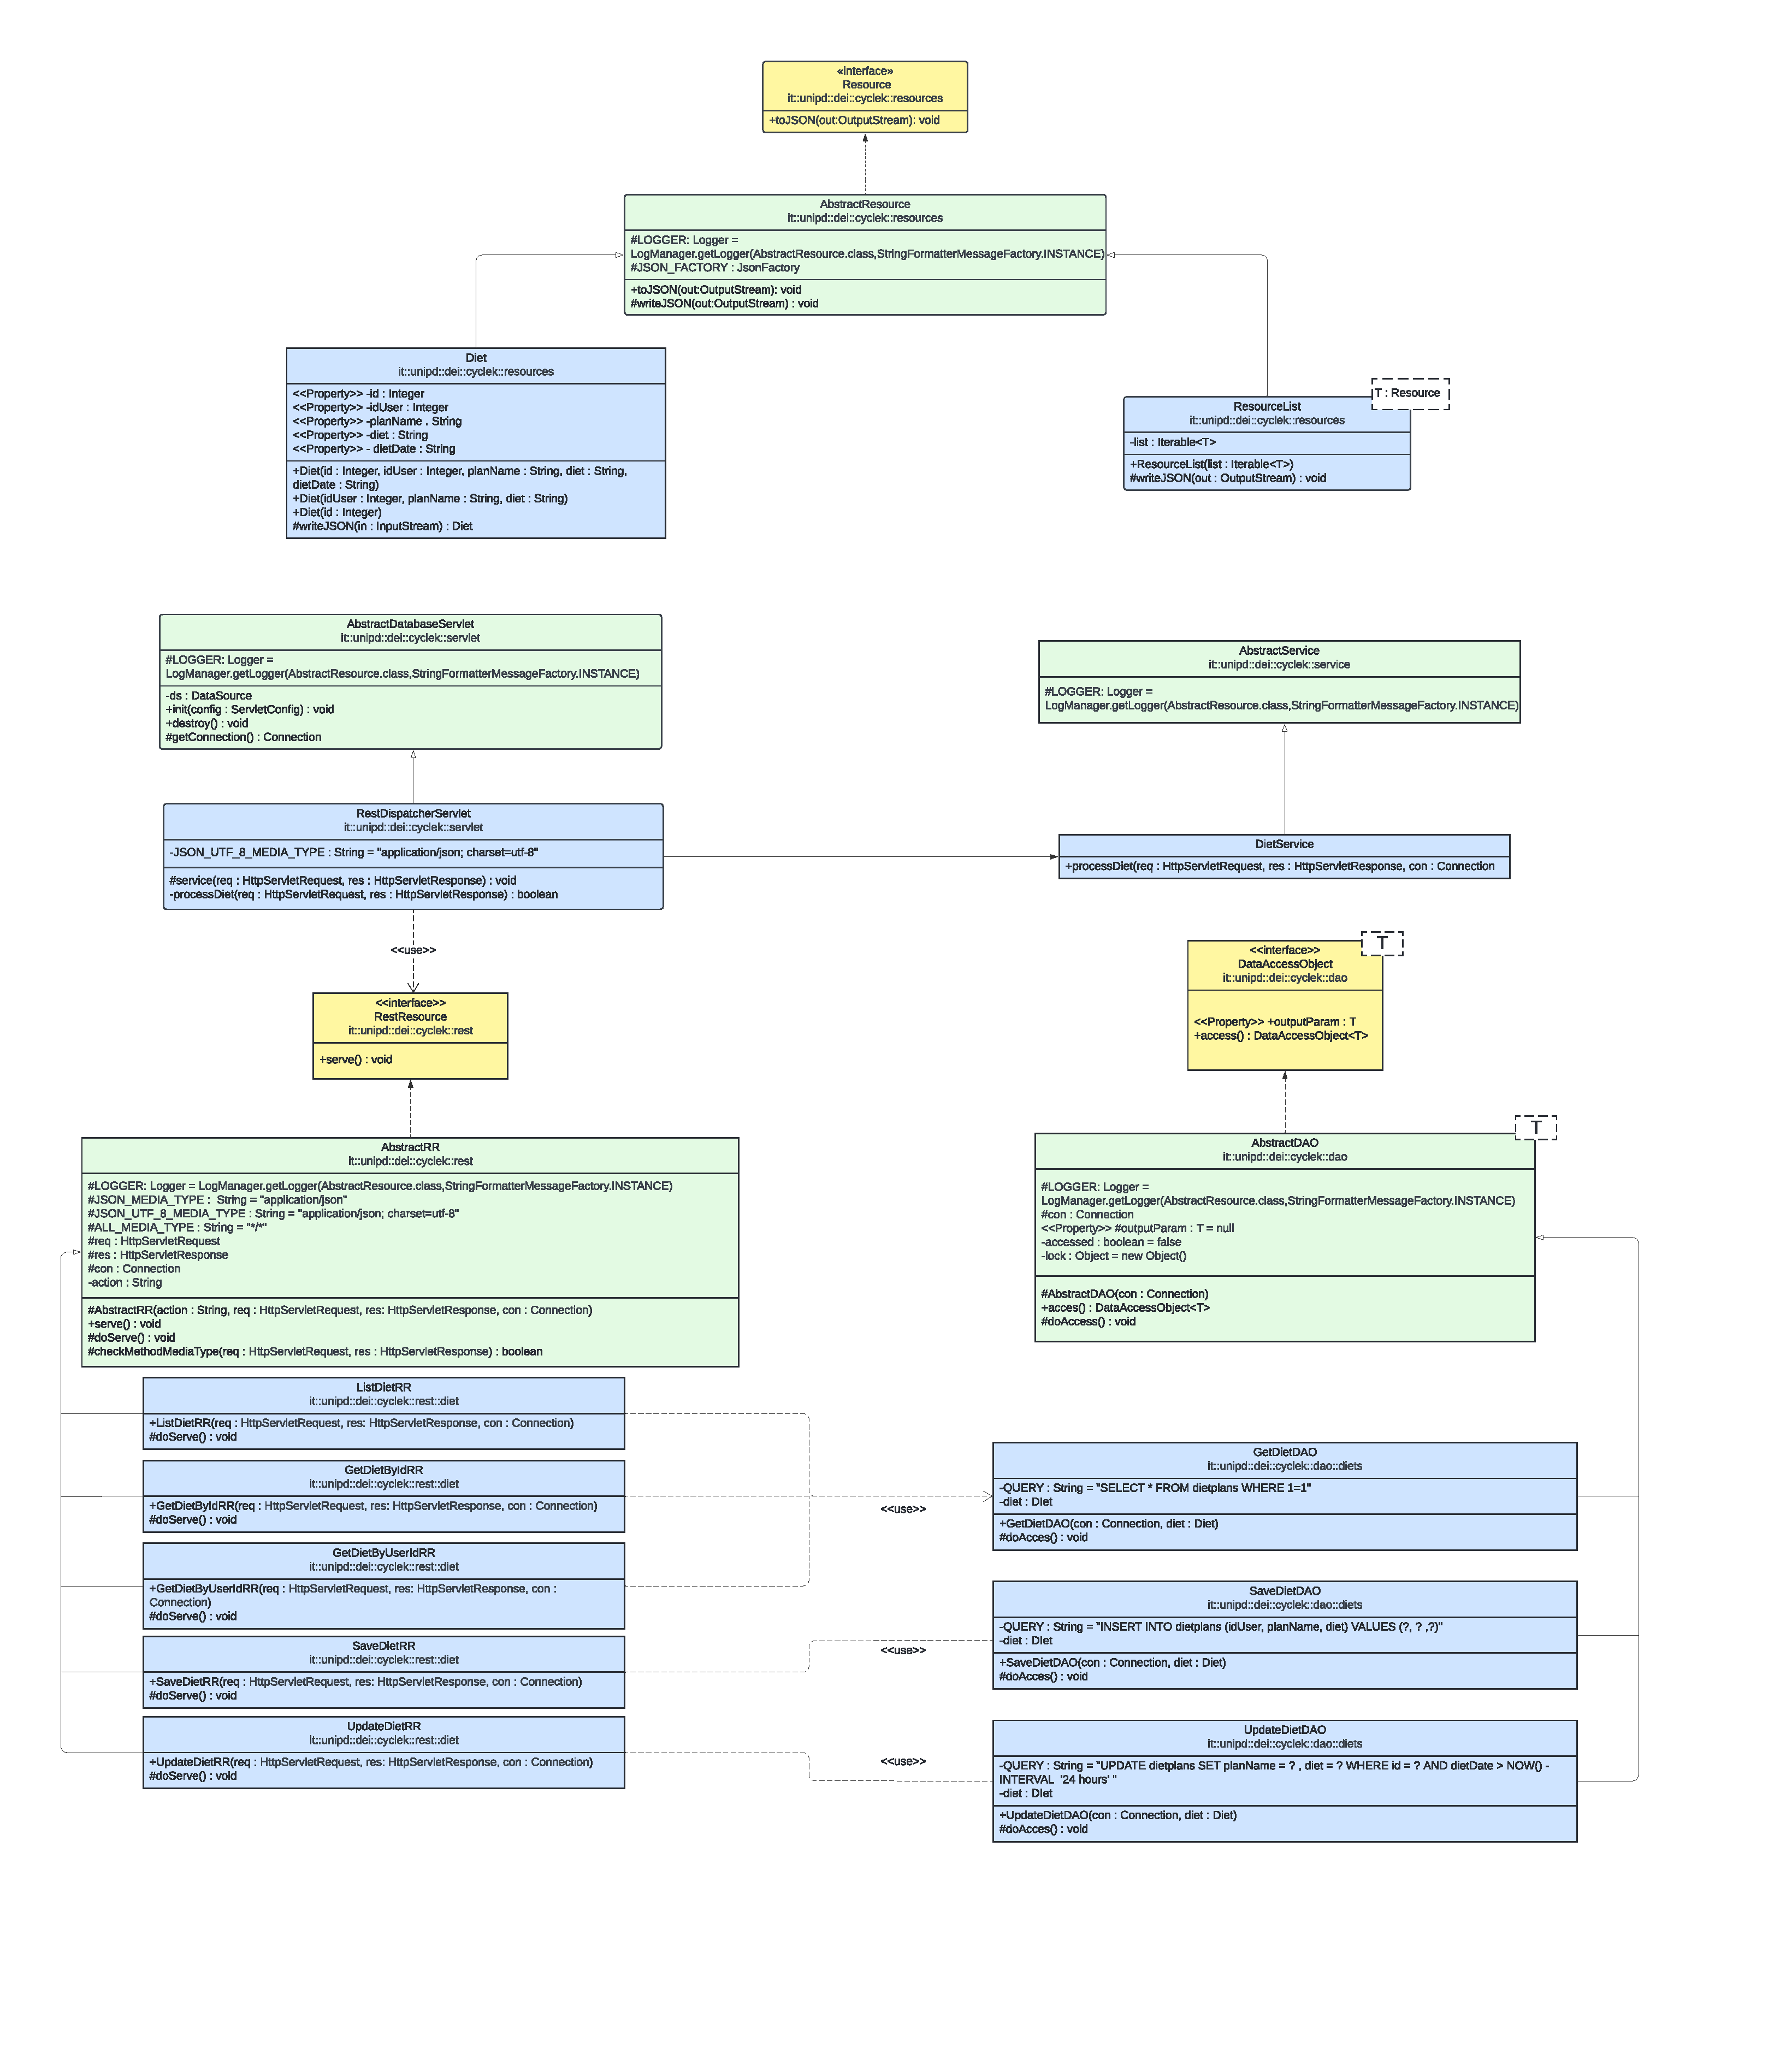
\includegraphics[scale=0.32]{Resources/DietUML.pdf}\newpage
%Describe here the class diagram of your project
The Class Diagram above depicts the diets resource. 
In the class diagram above, we can see the classes used to handle diet: creation, update, and loading. We have a resource called Diet which implements the constructors and the get methods for the parameters (which corresponds to the parameters in the ER schema). 
There is a \textit{RestDispatcherServlet} servlet that calls the corresponding rest resource (for example, if the request is a GET for user-specific diets , the \textit{RestDispatcherServlet} calls \textit{GetDietByUserIdRR}). Each one of these resources retrieves the parameters passed in \textit{JSON} format. After doing this, the rest resource calls the \textit{DAO} for the requested method. Then, the \textit{DAO} executes the \textit{SQL} statement and gets the data from the database. Then the \textit{DAO} returns the values requested.

The \textit{DAO}s for the creation of resources implement a \textit{POST} request;  for update implement a \textit{PUT} request; finally, the \textit{DAO}s for getting all diets and for getting the diet associated with the id, implement a \textit{GET} request.
\vspace{0.5 cm}
All the resources, are developed using \textit{REST}.

